\documentclass[10pt,paper=letter]{scrartcl}
\usepackage[alttitle]{cjquines}

\begin{document}

\title{VCSMS PRIME}
\subtitle{Program for Inducing Mathematical Excellence}
\author{Week 3 Homework}
\date{Due October 4, 2017}

\maketitle
\setlength{\unitlength}{1in}
\begin{picture}(0,0)
  \put(5.5,0.5){\hbox{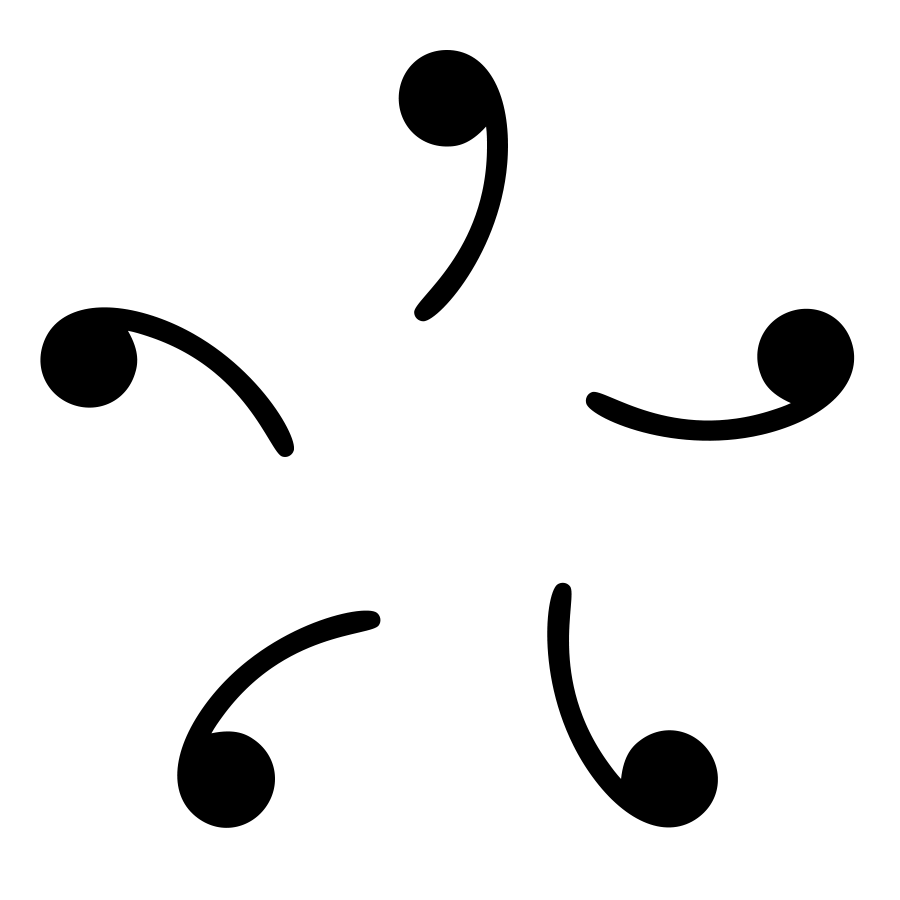
\includegraphics[width=0.9in]{logo.png}}}
\end{picture}
\vspace{-3.5em}

\subsubsection*{Homework}

Due on Wednesday, October 4. The additional problems this week are \emph{required} based on your set.

\begin{description}
  \item [Set A] (13) \textbf{S2}: Circular functions 1--2; Identities 1--2; Triangle laws 1--2.\\ \textbf{S7}: Circles 1--3; Three-dimensional 1. \textbf{Additional problems}: 1--3.
  \item [Set B] (13) \textbf{S2}: Circular functions 3--4; Identities 3; Equations 1--2; Triangle laws 3.\\\textbf{S7}: Circles 4--5; Three-dimensional 2--3. \textbf{S9}: Ad hoc 1; Triangles 1. \textbf{Additional problems}: 4.
  \item [Set C] (13) \textbf{S2}: Identities 4--5, 7; Equations 3--6; Triangle laws 4.\\ \textbf{S7}: Circles 6; Three-dimensional 4. \textbf{S9}: Ad hoc 2; Triangles 2. \textbf{Additional problems}: 5.
  \item [Set D] (13) \textbf{S2}: Identities 6; Equations 7--8; Triangle laws 5--6.\\ \textbf{S7}: Three-dimensional 5. \textbf{S9}: Ad hoc 3--5; Triangles 3--5. \textbf{Additional problems}: 6.
\end{description}

\subsubsection*{Additional problems}

Again, the additional problems this week are \emph{required}. Set A has 1--3, set B has 4, set C has 5 and set D has 6.

\begin{enumerate}

  \item Vincent is solving a problem: ``Two circles have radii $3$ and $27$, and the length of a common external tangent is $40$. What is the distance of their centers?'' However, he misread and thought it was ``common \emph{internal}'' tangent, and answered the problem correctly assuming this. What is the difference between Vincent's answer and the actual correct answer?

  \item (AIME 1994/2) A circle with diameter $PQ$ of length $10$ is internally tangent at $P$ to a circle of radius $20$. Square $ABCD$ is constructed with $A$ and $B$ on the larger circle, $CD$ tangent to $Q$ to the smaller circle, and the smaller circle outside $ABCD$. Find the length of $AB$.

  \item (AIME 1991/2) Rectangle $ABCD$ has $AB = 4$ and $CB = 3$. Divide $AB$ into $168$ congruent segments with points $A = P_0, P_1, \ldots, P_{168} = B$, and divide $CB$ into $168$ congruent segments with $C = Q_0, Q_1, \ldots, Q_{168} = B$. For $1 \leq k \leq 167$, draw the segments $P_kQ_k$. Repeat this construction on the sides $AD$ and $CD$, and then draw the diagonal $AC$. Find the sum of the lengths of the $335$ parallel segments drawn.

  \item (AHSME 1970) In trapezoid $ABCD$, we have $AB||CD$ and $\angle B = 2\angle D$. The length of $AB$ can be represented as $k$ times the length of $AD$ plus $\ell$ times the length of $CD$. What is $k + \ell$?

  \item (AIME 1998/6) Let $ABCD$ be a parallelogram. Extend $DA$ through $A$ to a piont $P$, and let $PC$ meet $AB$ at $Q$ and $DB$ at $R$. Given that $PQ = 735$ and $QR = 112$, find $RC$.

  \item A quadrilateral circumscribed about a circle has two adjacent right angles. The sides adjacent to one right angle have lengths $4$ and $7$. Find the radius of the inscribed circle.
\end{enumerate}

\subsubsection*{Additional reading}

\begin{itemize}
  \item Complex Numbers in Trigonometry, \url{https://aops.com/community/c6h609795}.

  \item Characterizations of Trapezoids, \url{http://forumgeom.fau.edu/FG2013volume13/FG201305.pdf}.
\end{itemize}

\end{document}
